\documentclass[11pt,spanish,a4paper]{article}
% Versión 2.o cuat 2014 Víctor Bettachini < bettachini@df.uba.ar >

\usepackage{babel}
\addto\shorthandsspanish{\spanishdeactivate{~<>}}
\usepackage[utf8]{inputenc}
\usepackage{float}

\usepackage{units}
\usepackage[separate-uncertainty=true, multi-part-units=single, locale=FR]{siunitx}

\usepackage{amsmath}
\usepackage{amstext}
\usepackage{amssymb}

% \usepackage{enumerate}

\newcommand{\pvec}[1]{\vec{#1}\mkern2mu\vphantom{#1}}

\usepackage{tikz}
\usepackage{xparse}
\usetikzlibrary{calc}

\tikzset{%
    Cote node/.style={%
        midway,
        sloped,
        fill=white,
        inner sep=1.5pt,
        outer sep=2pt
    },
    Cote arrow/.style={%
        <->,
        >=latex,
        very thin
    }
}

\makeatletter
\NewDocumentCommand{\Cote}{%
    s       % cotation avec les flèches à l'extérieur
    D<>{1.5pt} % offset des traits
    O{.75cm}    % offset de cotation
    m       % premier point
    m       % second point
    m       % étiquette
    D<>{o}  % () coordonnées -> angle
            % h -> horizontal,
            % v -> vertical
            % o or what ever -> oblique
    O{}     % parametre du tikzset
    }{%

    {\tikzset{#8}

    \coordinate (@1) at #4 ;
    \coordinate (@2) at #5 ;

    \if #7v % Cotation verticale
        \coordinate (@0) at ($($#4!.5!#5$) + (#3,0)$) ; 
        \coordinate (@4) at (@0|-@1) ;
        \coordinate (@5) at (@0|-@2) ;
    \else
    \if #7h % Cotation horizontale
        \coordinate (@0) at ($($#4!.5!#5$) + (0,#3)$) ; 
        \coordinate (@4) at (@0-|@1) ;
        \coordinate (@5) at (@0-|@2) ;
    \else % cotation encoche
    \ifnum\pdfstrcmp{\unexpanded\expandafter{\@car#7\@nil}}{(}=\z@
        \coordinate (@5) at ($#7!#3!#5$) ;
        \coordinate (@4) at ($#7!#3!#4$) ;
    \else % cotation oblique    
        \coordinate (@5) at ($#5!#3!90:#4$) ;
        \coordinate (@4) at ($#4!#3!-90:#5$) ;
    \fi\fi\fi

    \draw[very thin,shorten >= #2,shorten <= -2*#2] (@4) -- #4 ;
    \draw[very thin,shorten >= #2,shorten <= -2*#2] (@5) -- #5 ;

    \IfBooleanTF #1 {% avec étoile
    \draw[Cote arrow,-] (@4) -- (@5)
        node[Cote node] {#6\strut};
    \draw[Cote arrow,<-] (@4) -- ($(@4)!-6pt!(@5)$) ;   
    \draw[Cote arrow,<-] (@5) -- ($(@5)!-6pt!(@4)$) ;   
    }{% sans étoile
    \ifnum\pdfstrcmp{\unexpanded\expandafter{\@car#7\@nil}}{(}=\z@
        \draw[Cote arrow] (@5) to[bend right]
            node[Cote node] {#6\strut} (@4) ;
    \else
    \draw[Cote arrow] (@4) -- (@5)
        node[Cote node] {#6\strut};
    \fi
    }}
    }
\makeatother

\usetikzlibrary{decorations.pathmorphing, patterns}

\usepackage{graphicx}
\graphicspath{{./graphs_continuo/}}

\voffset-3.5cm
\hoffset-3cm
\setlength{\textwidth}{17.5cm}
\setlength{\textheight}{27cm}

\usepackage{lastpage}
\usepackage{fancyhdr}
\pagestyle{fancyplain}
\fancyhead{}
\fancyfoot{}
\fancyfoot[C]{ {\tiny Actualizado al \today} }
\fancyfoot[RO, LE]{Pág. \thepage/\pageref{LastPage}}
\renewcommand{\headrulewidth}{0pt}
\renewcommand{\footrulewidth}{0pt}


\begin{document}
\begin{center}
\textbf{Física 2} (Físicos) \hfill \textcopyright {\tt DF, FCEyN, UBA}\\
	% \textsc{\large Física 2 (Físicos)} - Prof. Diana Skigin - 2"o cuat. 2014\\
%	\textsc{\large Primer Cuatrimestre - 2014}\\
	\textsc{\LARGE Propagación de ondas en medios continuos}
	% \textsc{\large Guía 2:} Propagación de ondas en medios continuos
\end{center}



\begin{enumerate}

\item Verifique si las siguientes expresiones matemáticas cumplen la ecuación
de las ondas unidimensional. Grafique las funciones dadas.
\begin{itemize}
\item $\Psi(x,t)=Ae^{-\lambda(x-vt)^{2}}$
\item $\Psi(x,t)=\beta(x+vt)$
\item $\Psi(x,t)=A\sin\left[k(x-vt)\right]$
\item $\Psi(x,t)=B\sin^{2}\left(kx-\omega t\right)$
\item $\Psi(x,t)=C\cos(kx)\sin(\omega t)$
\item $\Psi(x,t)=De^{i(kx-\omega t)}$
\end{itemize}


\section*{Propagación en medios no dispersivos}

\item Se tiene una perturbación que se propaga en una cuerda infinita con
velocidad $v$. Se toman dos ``fotografías'' de la perturbación, a
$t=0$ s y $t=4$ s:
\begin{figure}[H]
\centering{}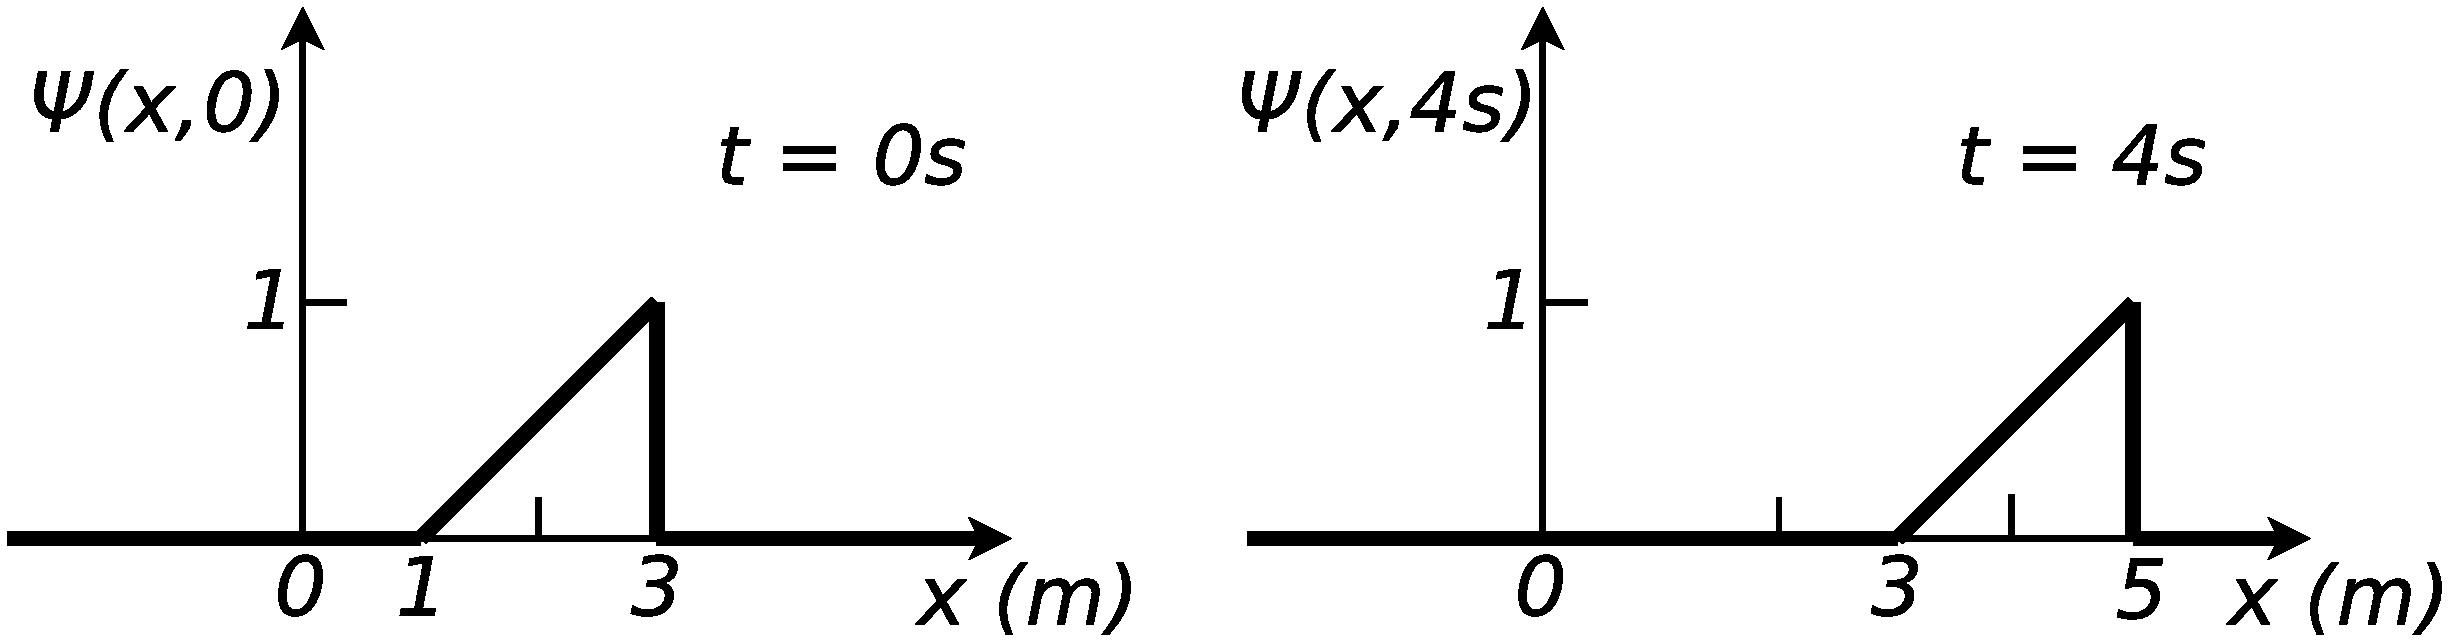
\includegraphics[clip,scale=0.25]{ej2-2}
\end{figure}
\begin{enumerate}
\item Hallar $v$.
\item Hallar $\Psi(x,t)$.
\end{enumerate}


\item Se tiene una cuerda infinita. Se sabe que la velocidad de propagación
de las ondas en ella es $v=100$ m/s (consideramos que dicha cuerda
es un medio no dispersivo). A $t=0$ se la deforma de la manera que
se indica en la figura, y se la suelta (desde el reposo).
\begin{figure}[H]
\centering{}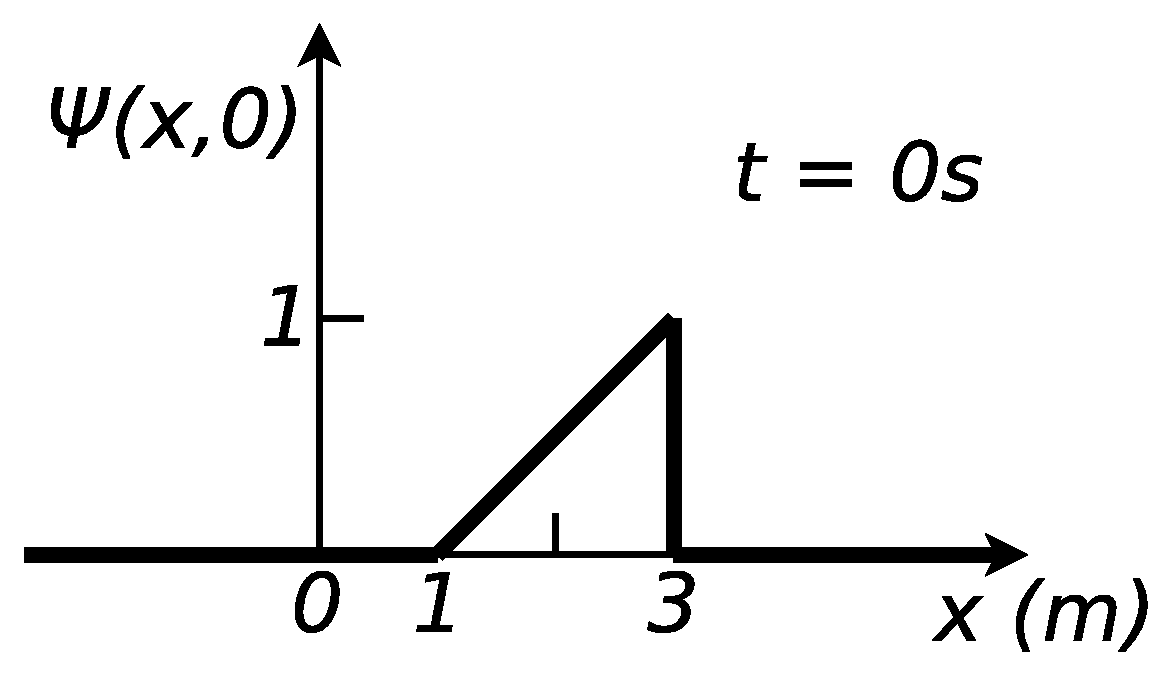
\includegraphics[clip,scale=0.25]{ej2-3}
\end{figure}
\begin{enumerate}
\item Hallar $\Psi(x,t)=\Psi_{1}(x-vt)+\Psi_{2}(x+vt)$. Dar explícitamente
(en cada intervalo de interés) la expresión de $\Psi(x,t)$.
\item Comparar esta situación con la del problema anterior.
\end{enumerate}


\item Se tiene una cuerda homogénea de longitud $L$ y densidad $\mu$,
a una tensión $T$, con sus dos extremos fijos $(x=0\mbox{ y }x=L)$.
A $t=0$ se la perturba de forma tal que
\[
\Psi(x,0)=\begin{cases}
0 & \mbox{si }0<x<a\\
h\frac{x-a}{L/2-a} & \mbox{si }a<x<L/2\\
h\frac{L-a-x}{L/2-a} & \mbox{si }L/2<x<L-a\\
0 & \mbox{si }L-a<x<L.
\end{cases}
\]
Se suelta la cuerda desde el reposo; considerar $h\ll L$.
\begin{enumerate}


\item Hallar $\Psi(x,t)$ y demostrar que siempre es posible escribir esta
solución como una superposición de una onda que se propaga hacia la
derecha y una que se propaga hacia la izquierda.
\item Hacer un esquema cualitativo del movimiento de la cuerda para los
instantes $t_{n}=n\frac{L}{8v}$, donde $v$ es la velocidad de propagación
de las ondas en la cuerda y $n$ es un número natural.
\end{enumerate}


\item En un gas, a $t=0$, se produce la perturbación indicada en la figura.
Sabiendo que $(\rho_{1}-\rho_{0})/\rho_{0}\ll1$ y que $v(x,0)=0$,
calcule $\rho(x,t)$.
\begin{figure}[H]
\centering{}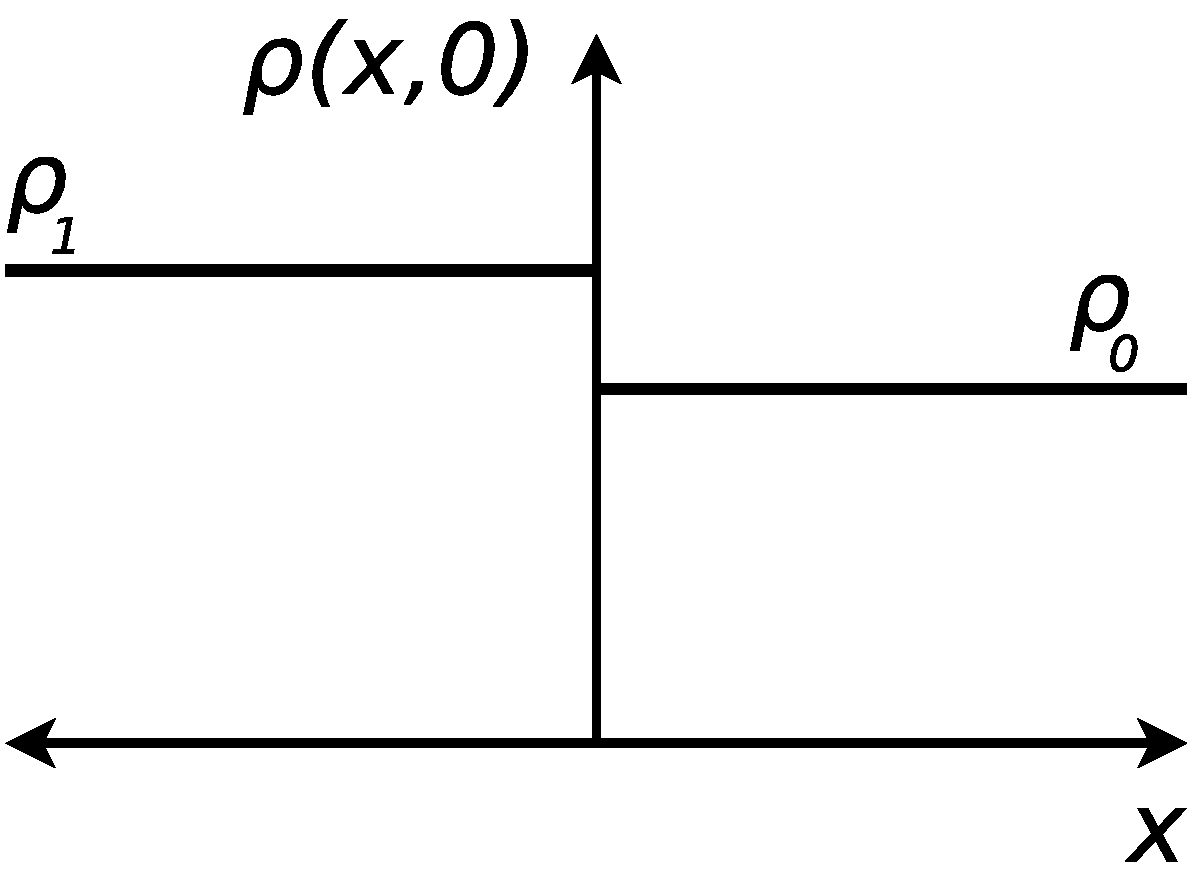
\includegraphics[clip,scale=0.25]{ej2-5}
\end{figure}
\begin{description}
\item [{Datos:}] $\rho_{1}$, $\rho_{0}$, $v_{s}$ (velocidad de propagación
de las ondas en el gas).
\end{description}


\section*{Ecuación de onda}

\item La ecuación de una onda transversal en una cuerda está dada por: $y(x,t)=0,1\unit{\, m}\sin\left[\pi\left(x\unit{\, m^{-1}-4\unit{\, s^{-1}}}\right)\right]$
($x$ e $y$ en metros y $t$ en segundos). Determine:
\begin{enumerate}
\item La amplitud de la onda.
\item La frecuencia de vibración de la cuerda.
\item La velocidad de propagación de la onda.
\item En $t=1$ s, evaluar el desplazamiento, la velocidad y la aceleración
de un segmento pequeño de cuerda ubicado en $x=2$ m.
\end{enumerate}


\item Sea una onda transversal plana y armónica, cuya frecuencia angular
vale $\omega=10\mbox{ s}^{-1}$ y cuyo número de onda es $k=100\mbox{\,\ m}^{-1}$.
En $x_{1}=1$ km y $t_{1}=1$ s la fase de la onda es $\nu(1\unit{\, km},1\unit{\, s})=3\pi/2$.
\begin{enumerate}
\item ¿Cuánto vale la fase en $x_{1}$ para $t=0$ s?
\item Considerando que $\nu(x,t)=kx-\omega t+\nu_{0}$, ¿cuánto vale $\nu_{0}$?
\item ¿A qué velocidad se propaga la onda?
\item ¿Cuánto tiempo debe transcurrir para que el frente de onda que se
hallaba en $x_{1}$ llegue a $x=2x_{1}$?
\end{enumerate}


\item Una cuerda larga con $\mu=0.005$ kg/m se tensa aplicando una fuerza
de $0.25$ N. El extremo izquierdo se mueve hacia arriba y hacia abajo
con movimiento armónico simple de período $0.5$ s y amplitud $0.2$
m; se supone que la tensión permanece constante en todo el movimiento.
Encontrar:
\begin{enumerate}
\item La velocidad de la onda generada en la cuerda, la frecuencia y la
longitud de onda.
\item La expresión matemática para el desplazamiento: $y(x,t)$.
\item La energía cinética media por unidad de longitud, de una partícula
del medio.
\item La energía potencial media por unidad de longitud, de una partícula.
\end{enumerate}


\section*{Reflexión y transmisión de ondas}

\item Se tienen dos cuerdas semi--infinitas, de densidades lineales $\rho_{1}$
y $\rho_{2}$, unidas en un punto. El sistema está sometido a una
tensión $T$. Sobre la primera cuerda (la de densidad $\rho_{1}$)
incide una onda de la forma: $\phi_{i}(x,t)=A_{i}\cos\left(k_{1}x-\omega t\right)$.
Se conocen: $\rho_{1}$, $\rho_{2}$, $T$, $\omega$ y $A_{i}$.
\begin{enumerate}
\item Calcule $k_{1}$ y $k_{2}$, es decir, los números de onda de cada
lado de la unión.
\item Plantee la solución más general para $\phi(x,t)$ de cada lado de
la unión.
\item ¿Qué condiciones deben verificarse en el punto de unión de las cuerdas?
\item Usando (b) y (c), calcule la perturbación $\phi(x,t)$ en cada una
de las cuerdas.
\end{enumerate}


\item Se tienen dos caños semi-infinitos de distinta sección y unidos,
como se muestra en la figura. Una onda acústica de la forma $\delta p_{i}(x,t)=A_{i}\cos\left(k_{1}x-\omega t\right)$
incide desde el primer caño hacia $x>0$. Hallar las amplitudes de
presión y elongación de las ondas reflejadas y transmitidas.
\begin{figure}[H]
\centering{}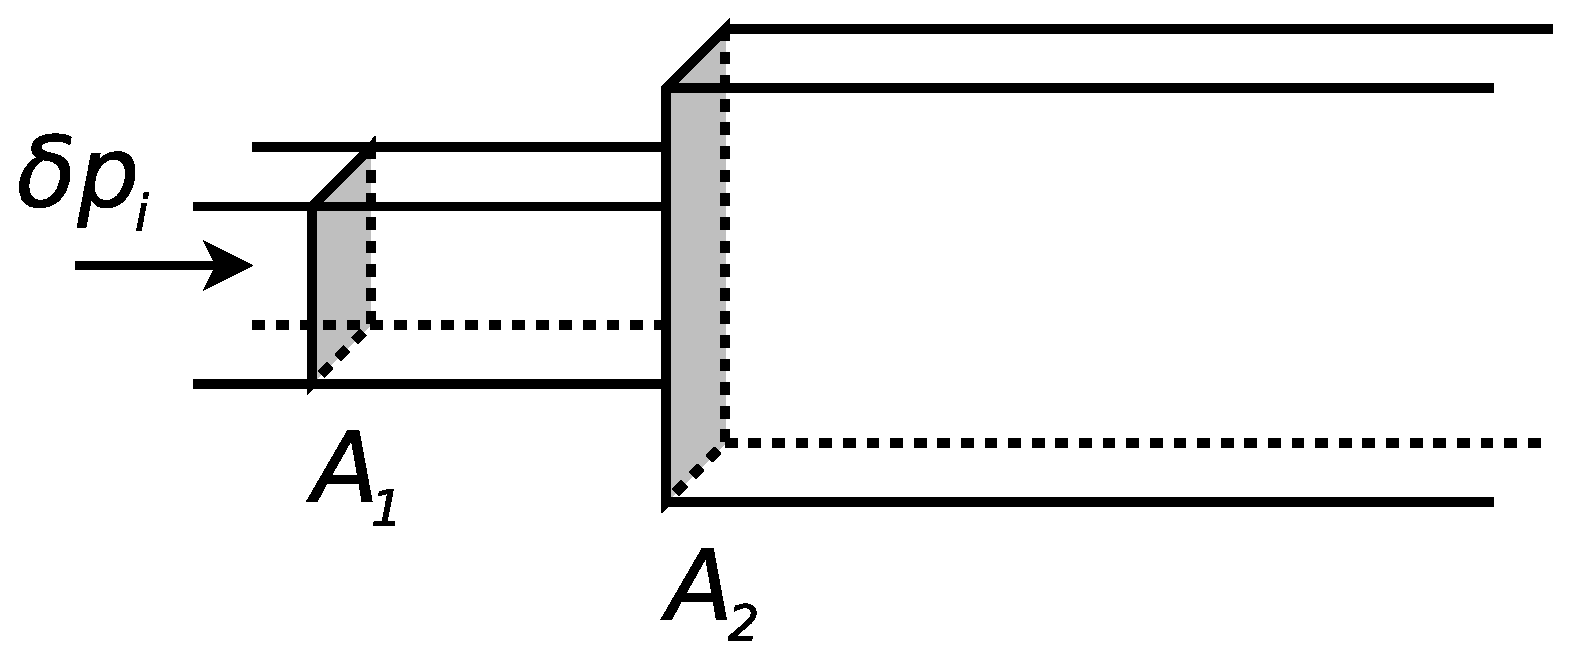
\includegraphics[clip,scale=0.25]{ej2-10}
\end{figure}
\begin{description}
\item [{Datos:}] $A_{1}$, $A_{2}$, presión media $P_{0}$, densidad media
$\rho_{0}$, $v_{s}$, $\omega$, $A_{i}$. Suponer despreciables
los efectos de la viscosidad.
\end{description}


\item Considere la siguiente configuración:
\begin{figure}[H]
\centering{}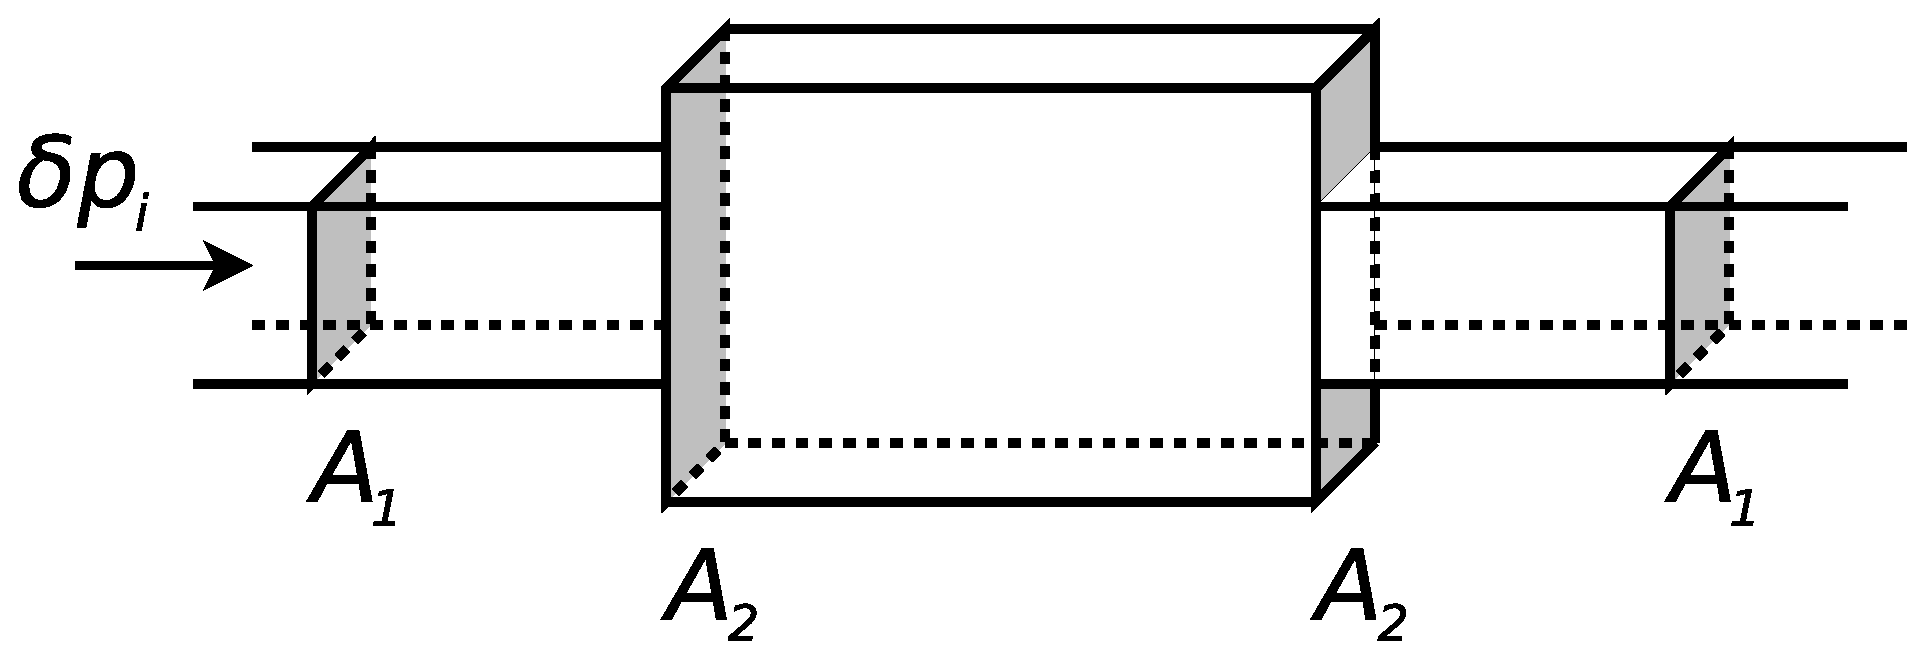
\includegraphics[clip,scale=0.25]{ej2-11}
\end{figure}
Suponga que desde la izquierda incide una onda cuya expresión es la
misma del problema anterior (las secciones y el resto de los datos
son los mismos también). Hallar $\delta p(x,t)$ y $\Psi(x,t)$ en
cada tramo.
\item Se tiene una interfase plana e infinita entre aire y agua (ver figura).
\begin{figure}[H]
\centering{}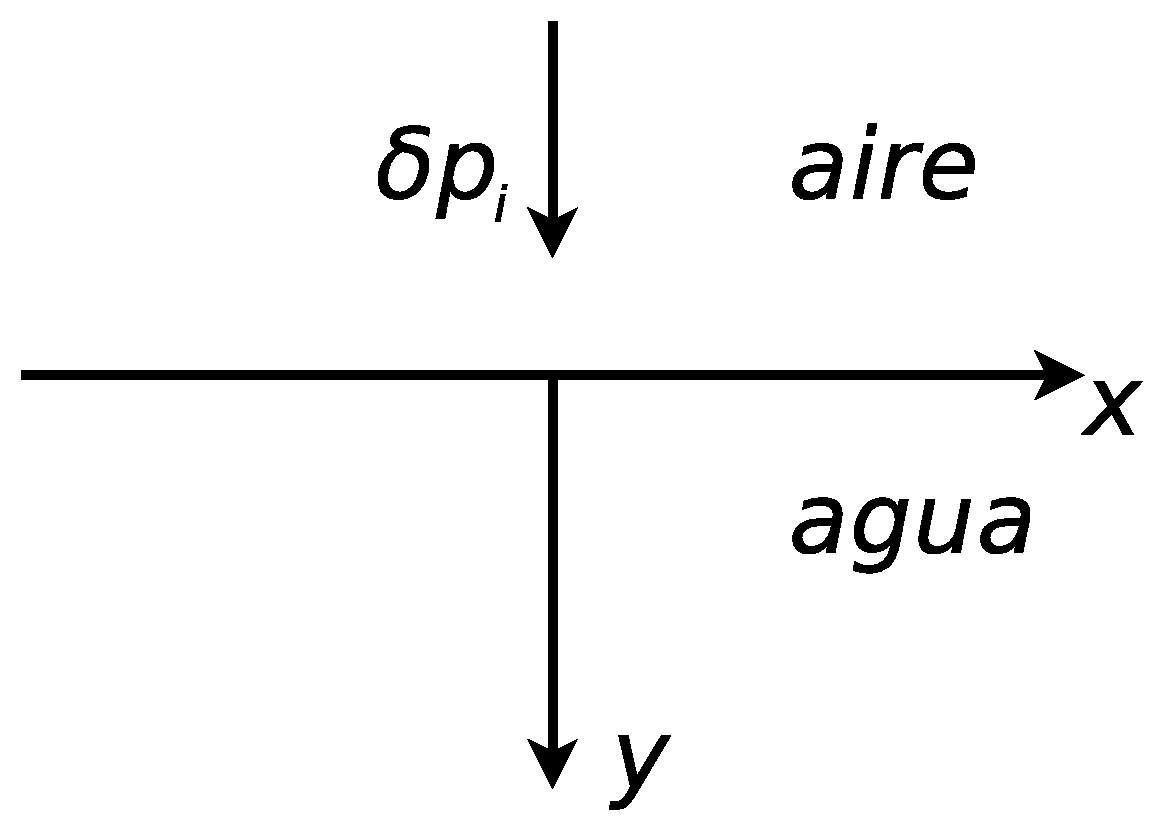
\includegraphics[clip,scale=0.25]{ej2-12}
\end{figure}
Desde el aire incide una onda acústica plana cuya dirección de propagación
es normal a la interfase; se escribe $\delta p_{i}(y,t)=A_{i}\cos\left(k_{1}y-\omega t\right)$.
Hallar las ondas reflejadas y transmitidas $\delta p_{r}(y,t)$ y
$\delta p_{t}(y,t)$.


\item 
\begin{enumerate}
\item Demuestre que la función: $\Psi(\mathbf{r},t)=Ae^{i(\mathbf{k}\cdot\mathbf{r}\pm\omega t)}$,
con $\mathbf{k}=k_{x}\hat{x}+k_{y}\hat{y}+k_{z}\hat{z}$ un vector
constante y $\mathbf{r}=x\hat{x}+y\hat{y}+z\hat{z}$, es solución
de la ecuación de ondas tridimensional. Sugerencia: exprese el laplaciano
en coordenadas cartesianas.
\item Analice el significado físico de $\Psi(\mathbf{r},t)$. ¿Cómo son
los frentes de onda? ¿Cuál es la relación entre el vector $\mathbf{k}$
y los frentes de onda? ¿Hacia dónde se desplazan los frentes de onda
al transcurrir $t$? ¿A qué velocidad?
\item Rehaga el problema anterior suponiendo que la onda incidente (desde
el aire) forma un ángulo $\theta$ con la normal a la interfase (ver
figura).
\begin{figure}[H]
\centering{}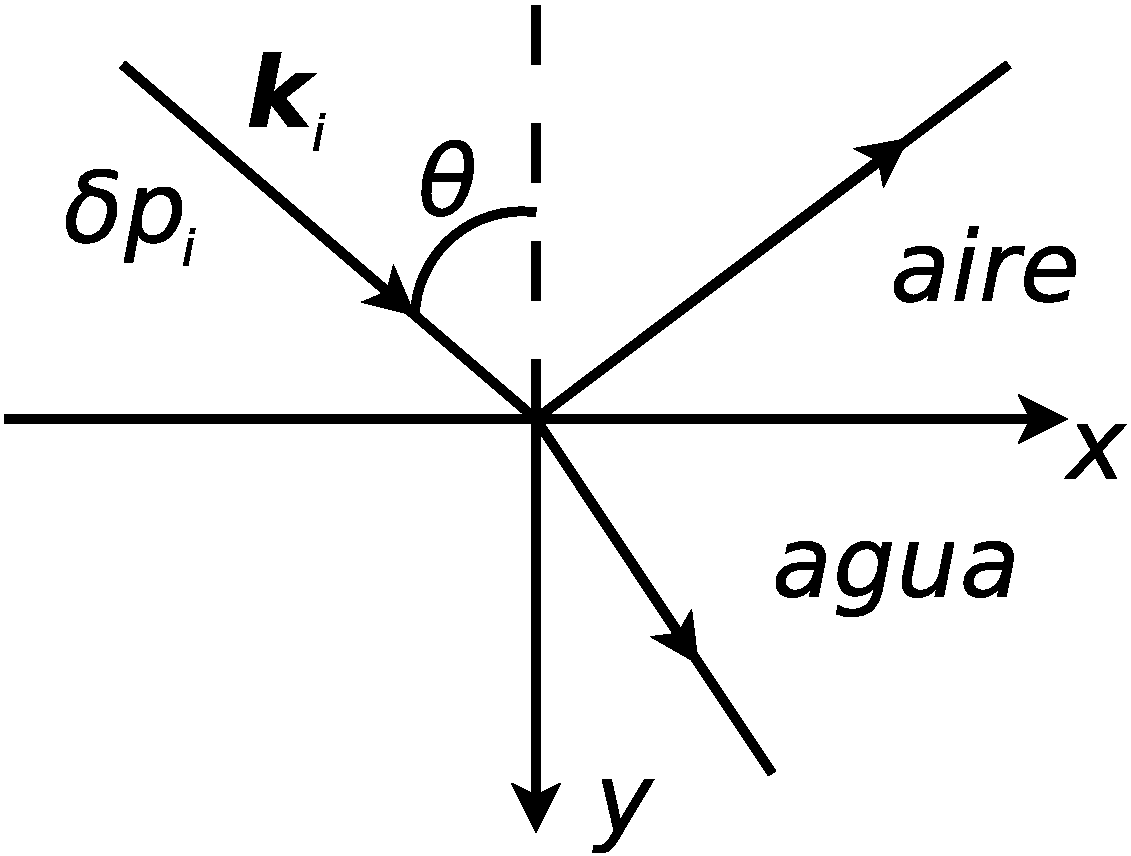
\includegraphics[clip,scale=0.25]{ej2-13}
\end{figure}
 Por lo tanto la onda de presión incidente se escribe, si usamos notación
 compleja: $\delta p_{i}(\mathbf{r},t)=A_{i}e^{i(\mathbf{k}_{i}\cdot\mathbf{r}-\omega t)}$,
 siendo $\mathbf{k}_{i}=\frac{\omega}{v_{s}}\left(\sin\theta\hat{x}+\cos\theta\hat{y}\right)$.
 Hallar las ondas reflejadas y transmitidas, $\delta p_{r}(\mathbf{r},t)=A_{r}e^{i(\mathbf{k}_{r}\cdot\mathbf{r}-\omega t)}$
 y $\delta p_{t}(\mathbf{r},t)=A_{t}e^{i(\mathbf{k}_{t}\cdot\mathbf{r}-\omega t)}$.
\end{enumerate}



\section*{Velocidad de fase y velocidad de grupo}

\item En lo que sigue, encuentre con cuál de estos métodos se determina
 la velocidad de fase y con cuál la de grupo.
\begin{enumerate}
\item Medir la velocidad del sonido en el aire, golpeando las manos y determinando
el tiempo que transcurre entre el aplauso y el eco de un reflector
ubicado a una distancia conocida.
\item Medir la longitud de un tubo que resuena a una frecuencia conocida
(y corregir por efectos de borde).
\item Determinar la velocidad de la luz midiendo el tiempo que tarda un
haz colimado en recorrer una distancia conocida.
\item Encontrar la longitud de una cavidad resonante que oscila en un modo
conocido a una frecuencia conocida.
\end{enumerate}


\item Demuestre que la velocidad de grupo $v_{g}$ y la velocidad de fase
$v_{f}$ están relacionadas por:
\[
v_{g}=v_{f}-\lambda\frac{dv_{f}}{d\lambda}
\]
¿Cómo es $\frac{dv_{f}}{d\lambda}$ en un medio no dispersivo? En
ese caso, ¿cómo se relacionan la velocidad de grupo y la de fase?


\section*{Trasformada de Fourier}

\item Se quiere investigar la relación entre el ancho de un paquete y el
desfasaje de las frecuencias que lo componen.
\begin{enumerate}
	\item Tome el siguiente pulso con un espectro gaussiano de ancho $\Delta k$
centrado en $k_{0}$ (note que las frecuencias están en fase):
\[
F(k)=A\exp\left[-\frac{(k-k_{0})^{2}}{4\Delta k^{2}}\right].
\]
Calcule $f(x)$ y vea que tiene una envolvente gaussiana que modula
una portadora de frecuencia $k_{0}$. Note que el pulso está centrado
en $x=0$ y que se cumple la relación $\Delta x\Delta k=1/2$ (el
paquete gaussiano es el de mínima incerteza).
	\item Ahora desfase las distintas frecuencias en forma lineal, tal que:
\[
F(k)=A\exp\left[-\frac{(k-k_{0})^{2}}{4\Delta k^{2}}\right]\exp\left[i\alpha(k-k_{0})\right].
\]
Calcule $f(x)$ y vea que es el mismo pulso que en la parte (a), pero
desplazado en $\alpha$ hacia la derecha (una fase lineal sólo corre
la función).
	\item Ahora agregue una fase cuadrática, es decir:
\[
F(k)=A\exp\left[-\frac{(k-k_{0})^{2}}{4\Delta k^{2}}\right]\exp\left[i\beta(k-k_{0})^{2}\right].
\]
Calcule $f(x)$ y vea que es un pulso gaussiano centrado en $x=0$
pero con un ancho $\Delta x$ que cumple:
\[
\Delta x\Delta k=\frac{1}{2}\sqrt{1+16\beta^{2}\Delta k^{4}}.
\]
¿Es cierto que si se quiere disminuir el ancho de un paquete siempre
se debe aumentar $\Delta k$? Derive $\Delta x$ con respecto a $\Delta k$
de la expresión anterior y analice lo pedido.
\end{enumerate}
\begin{description}
	\item [{Ayuda:}] $\int_{-\infty}^{+\infty}\exp\left[-(\alpha x)^{2}\right]dx=\sqrt{\frac{\pi}{\alpha}}$.
\end{description}



% Espectro cuadrado
\item Si $\Psi(\omega)$ corresponde a un espectro de frecuencias cuadrado,
o sea $\Psi(\omega)=1/\Delta\omega$ para $\omega$ comprendida en
el intervalo de ancho $\Delta\omega$ alrededor de $\omega_{0}$,
y cero en otra parte; vea que $\phi(t)$ está dada por:
\[
\phi(t)=\frac{1}{\sqrt{\pi}}\left[\frac{\sin(t\Delta\omega/2)}{t\Delta\omega/2}\right]e^{i\omega_{0}t}
\]
\begin{enumerate}
\item Grafique $\Psi(\omega)$ y $\left|\phi(t)\right|$.
\item Sea $T$ un tiempo más prolongado que la duración de cualquier experimento
que pueda idear. Muestre que si $\Delta\omega$ es suficientemente
pequeño como para que $\Delta\omega T\ll1$, entonces durante un tiempo
menor que $T$, $\phi(t)$ es una función armónica de amplitud y fase
casi constante.
\end{enumerate}


% Pulso cuadrado
\item Sea $\phi(t)$ una función real.
\begin{enumerate}
	\item Muestre que su transformada de Fourier $\Psi(\omega)$ cumple $\Psi(\omega)=\Psi(-\omega)$.
Use esto para escribir a $\phi(t)$ como superposición de senos y
cosenos.
	\item Muestre que la transformada de Fourier $\mathcal{F}$ es lineal, esto
quiere decir que
\[
\mathcal{F}(af+bg)=a\mathcal{F}(f)+b\mathcal{F}(g)
\]
donde $f$ y $g$ son funciones de $x$ y $a$ y $b$ son constantes.
	\item Tomemos una pulsación que se repite $N$ veces:
\begin{figure}[H]
\centering{}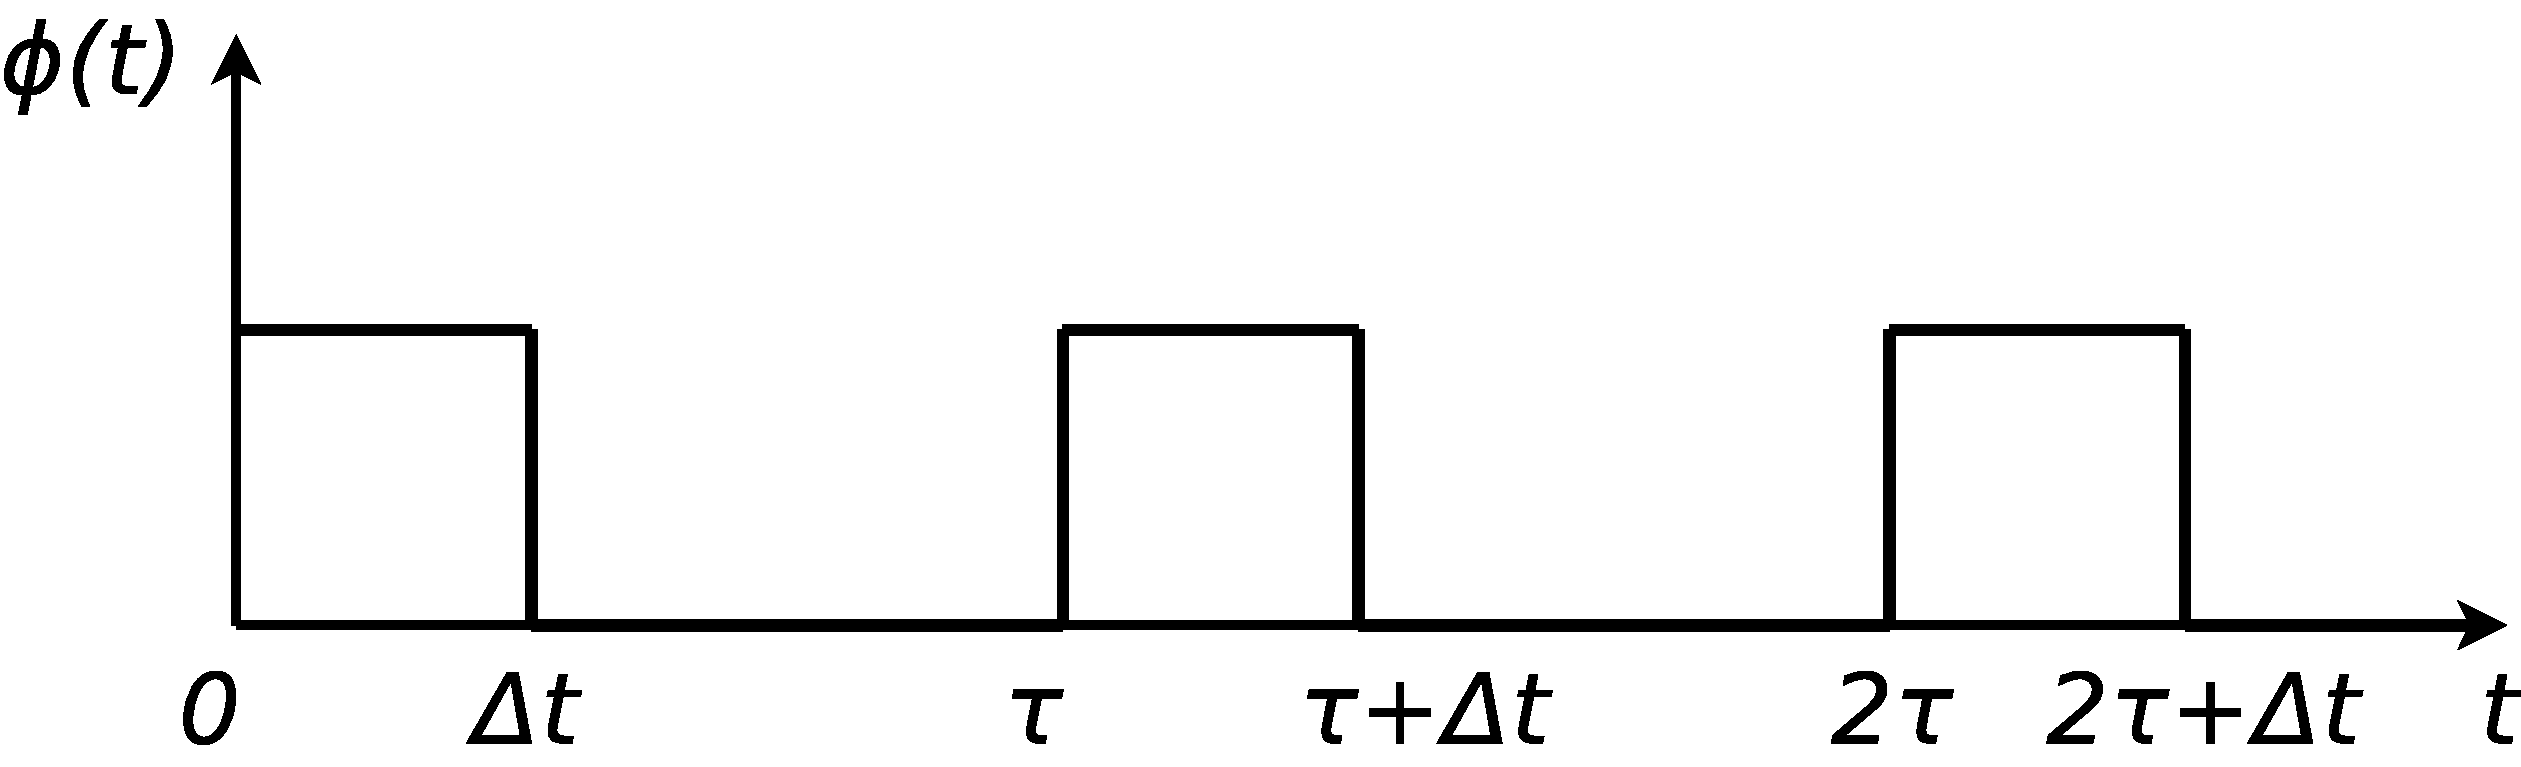
\includegraphics[clip,scale=0.25]{ej2-18}
\end{figure}
Vea que la transformada de Fourier de un único pulso situado entre
$(n\tau,n\tau+\Delta t)$ es igual a la transformada del pulso $(0,\Delta t)$
multiplicado por la fase $e^{in\phi}$. Calcule entonces la transformada
de la pulsación cuadrada que se repite en un tiempo largo $T_{largo}=N\tau$.
	\item Muestre que para un valor finito de $T_{largo}$ el análisis de Fourier
de esta pulsación cuadrada repetida casi periódicamente, consiste
en una superposición de armónicos casi discretos de la frecuencia
fundamental $\nu_{1}=1/T_{1}$, siendo realmente cada armónico un
continuo de frecuencias que se extiende sobre una banda de ancho $\delta\nu\approx1/T_{largo}$.
Las armónicas más importantes caen entre 0 y $\Delta\nu=1/\Delta t$.
	\item ¿Por qué vale $\Delta t\Delta\nu\approx1$ si, en principio, podría
valer $\Delta t\Delta\nu\gg1$? ¿La misma pregunta es aplicable a
$\delta\nu$ y $T_{largo}$?
\end{enumerate}


\section*{Progación en medios dispersivos}

\item Se tiene un pulso de ancho $\Delta k$ centrado en $k_{0}$ tal que
la siguiente es una buena aproximación para la relación de dispersión:
\[
\omega(k)=\omega_{0}(k_{0})+\omega'(k_{0})(k-k_{0})+\frac{1}{2}\omega''(k_{0})(k-k_{0})^{2}
\]
Si en $t=0$ el pulso se propaga hacia $x<0$, y se escribe:
\[
\Psi(x,0)=A\int_{-\infty}^{+\infty}\exp\left[-\frac{(k-k_{0})^{2}}{4\Delta k^{2}}\right]\exp\left(ikx\right)dk+c.c.
\]
Calcule $\Psi(x,t)$. Vea cuál es la posición y el ancho del paquete
como función del tiempo. ¿Es cierto que al viajar por un medio dispersivo
cualquier paquete se ensancha?


\item Se tienen dos cuerdas semi-infinitas de distinta densidad lineal
de masa, $\rho_{1}$ y $\rho_{2}$, unidas en un punto y sometidas
a una tensión $T$. Sobre la primera se propaga hacia la derecha una
perturbación de la forma indicada en la figura. Se conocen $\rho_{1}$,
$\rho_{2}$, $T$, $L$ y $h$. También se considera que los medios
son no dispersivos.
\begin{figure}[H]
\centering{}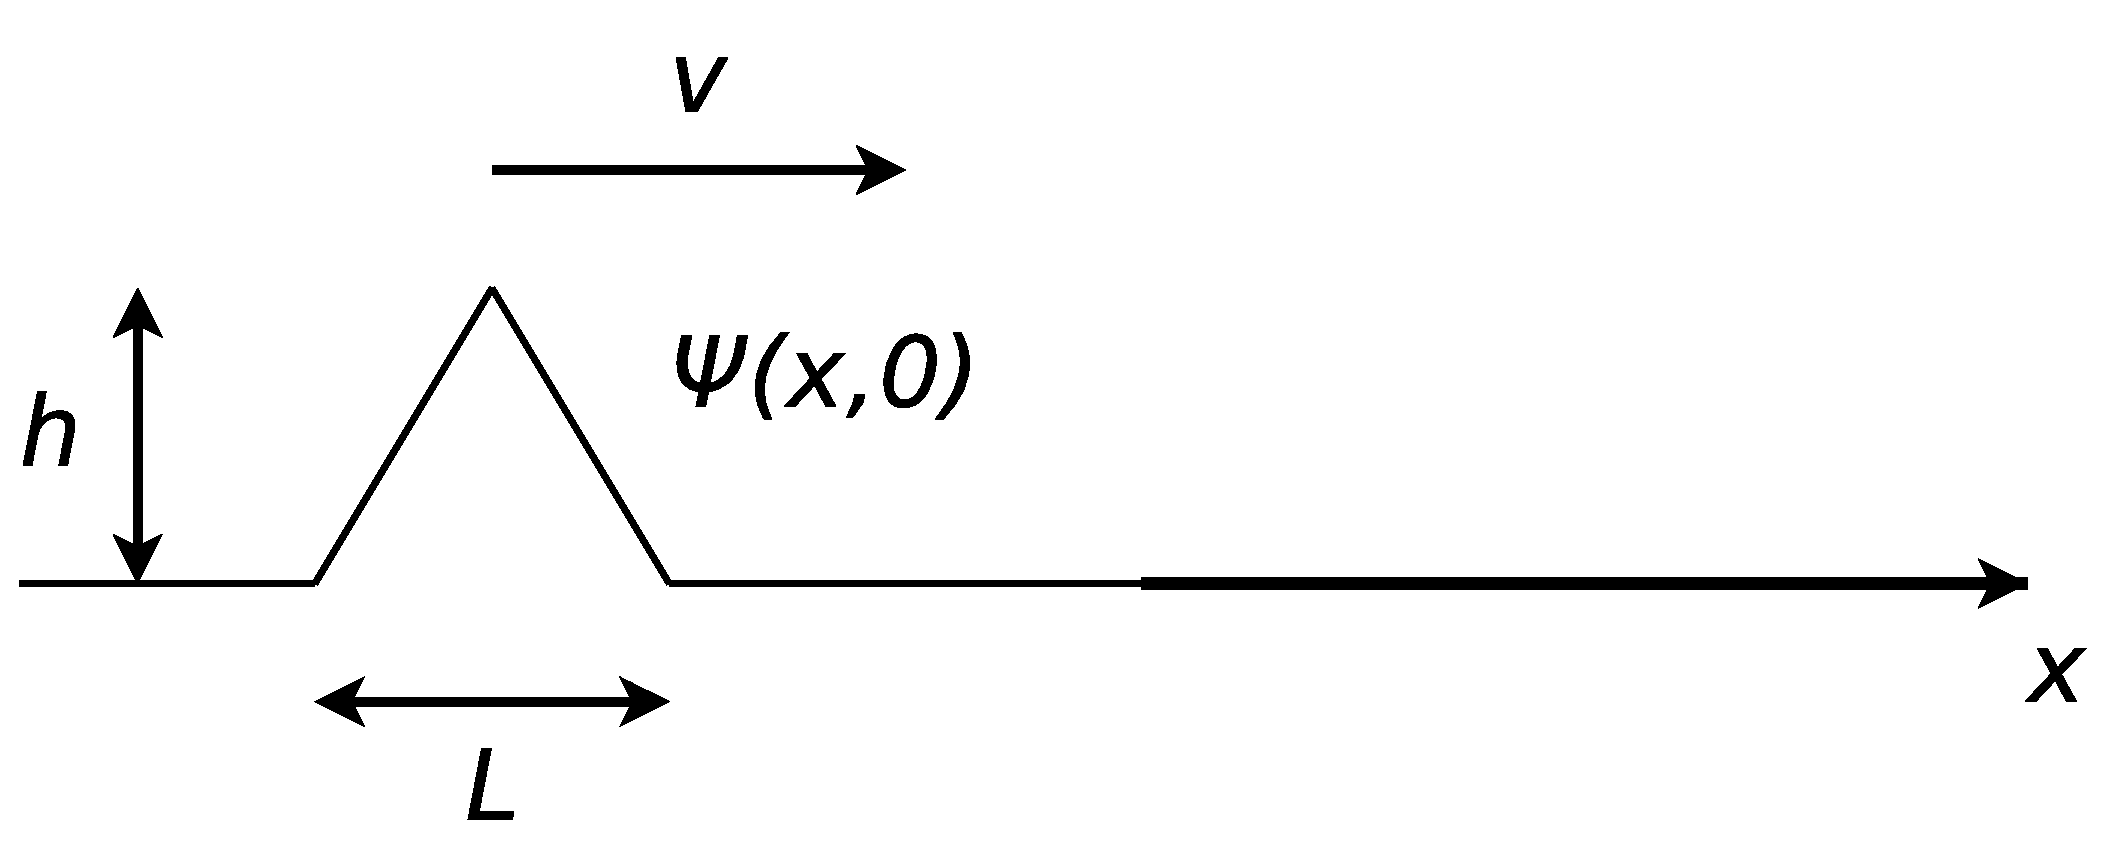
\includegraphics[clip,scale=0.25]{ej2-20}
\end{figure}
\begin{enumerate}
\item Hallar el desplazamiento $y(x,t)$.
\item Explique cualitativamente como cambian estos resultados si el medio
es dispersivo.
\end{enumerate}


\section*{Efecto Doppler | Ondas de choque}

\item \textbf{Efecto Doppler.} Una fuente de sonido que emite en una frecuencia
de 1000 Hz se mueve hacia la derecha a 40 m/s. Un observador, que
está a la derecha de la fuente, también se mueve hacia la derecha
a 20 m/s.
\begin{enumerate}
\item ¿Cuál será la frecuencia detectada por el observador? El aire se encuentra
en reposo.
\item Repita el punto anterior si hay viento hacia la derecha a 20 m/s.
\item Repita todo lo hecho si el observador se encuentra inicialmente a
la izquierda de la fuente.
\end{enumerate}



\item \textbf{Ondas de choque.} Un avión a retropropulsión en vuelo horizontal
a 5000 m de altura pasa sobre un observador con velocidad $2.2$ Mach
(o sea, $2.2$ veces la velocidad del sonido). Calcular:

\begin{enumerate}
\item El ángulo formado por el frente de la onda sonora y la dirección del
movimiento.
\item ¿Cuánto tiempo después de haber pasado el avión sobre el observador
la onda llega a éste?
\item Si el piloto hace sonar una bocina en el instante en que pasa justo
sobre el observador, ¿cuánto tiempo después escucha el observador
ese sonido?
\end{enumerate}



\end{enumerate}

\end{document}
